
\documentclass[authoryear,preprint,review,12pt]{elsarticle}

\usepackage{graphicx}
\graphicspath{{./figures/}}
\DeclareGraphicsExtensions{.pdf,.jpeg,.png,.jpg}

\usepackage{amssymb}
\usepackage{lineno}
\usepackage{natbib}
\usepackage{url}
\usepackage[utf8]{inputenc}
\usepackage{siunitx}

\journal{Veg Hist Archaeobot}

\begin{document}

\begin{frontmatter}

\title{Investigating fuel and fireplaces through a combination of phytoliths and multi-element analysis. An ethnographic experiment}

\author[label1,label2]{Carla Lancelotti}
\author[label1,label3]{Javier Ruiz-Pérez}
\author[label1,label4]{Juan José García-Granero}
\address[label1]{CaSEs - Complexity and Socio-Ecological Dynamics Research Group}
\address[label2]{Department of Humanities, Pompeu Fabra University, Barcelona (Spain)}
\address[label3]{Department of Animal and Plant Biology and Ecology, Faculty of Biosciences, Autonomous University of Barcelona, Barcelona (Spain)}
\address[label4]{Department of Archaeology and Anthropology, Instituciò Milà i Fontanals, Spanish Research Council (CSIC)}


\begin{abstract}
The determination of fuel-related practices in archaeological contexts is almost always associated to the identification of fire-related structures. Anthracological analysis is standard to identify wood use in the past; however, in many circumstances wood was not the primary source of fuel. In arid and semi-arid environments alternative fuels such as dung, chaff and straw and, in general, plant-processing byproducts are predominant. The study of these types of fuel often necessitates the application of multi-proxy analyses, involving botanical micro-remains and geochemistry.
This paper presents the results of an integrated analysis of phytoliths and chemical elements of samples collected in an ethnographic context (a domestic compound), in North Gujarat, India. Alternative fuels have been and are still very important in this area due to the scarcity of wood and the recent ban on cutting trees imposed by the Government. Within the house studied, three fireplaces are present where different types of activities are performed selectively. The differential use of fuels in the three fireplaces is highlighted by the results of descriptive and multivariate statistics. However, the opposite geochemical signals that the fireplaces produce would be difficult to interpret in an archaeological context where the practices that produced such signal are unknown. The combination of phytoliths and geochemistry, coupled with the ethnographic information on the activity, can help us to construct stronger models to interpret the archaeological record.
\end{abstract}

\begin{keyword}
fuel \sep phytoliths \sep ethnography \sep geochemistry \sep India \sep anthropic activity markers
\end{keyword}

\end{frontmatter}

\linenumbers

\section{Introduction}
\label{sec:1}
Fire-related contexts, whether built structures or remains of scattered ashes, are one of the most common features in archaeological contexts. These contexts offer detailed information on past activities, both domestic and industrial. Through the study of fire-related structures, archaeologists can gain insights on various aspects of human behaviour including technology, food consumption, resource use and indirectly, on some aspects of the landscape and ecology in which a particular society developed its activities \citep{Asouti2003,Chabal1997,Meyer2003,ShahackGross2004}. The identification of these contexts can sometimes be problematic, especially when the structure is not clearly identifiable during excavation. Very often, especially in urban societies, fire-related structures are easy to identify as they are built in permanent materials. On the contrary, in semi-permanent camps and small settlements (e.g. hunter-gatherer sites, pastoral camps, etc.) structures might not be easily identified. A common feature used to identify fireplaces in these contexts is the presence of rubified sediments surrounding the fireplace. However, as highlighted by micromorphological studies conducted in Jandhala, rubefaction is very limited in this contexts and the walls of the fireplaces show only minimal traces of it on their innermost face (Yannitto, V. 2011. \textit{Micromorfología en contexto etnoarqueológico. Técnicas constructivas entre los agricultores de Jhandala (Gujarat, India)}. Unpublished MPhil Dissertation). In addition, there exists a series of contexts whereby post-depositional processes hamper the identification of fire-related structures. We are here referring to all those situations in which the fire installation is built with the same materials that compose floors and walls (i.e. mudbrick and wattle-and-daub structures). In arid, semi-arid and, to a certain extent, temperate prehistoric and historic contexts buildings constructed of mudbricks are very common; however, our identification of such structures is hampered by their being extremely prone to degradation \citep{Friesem2014}.
Beyond the recognition of firing structures, a further problem in the identification of fuel-related practices is represented by the choice of fuel that people used in the past. Wood is beyond any doubt the most common fuel in temperate and tropical contexts, though bone has been identified in few cases as an alternative source of fuel \citep{Beresford-jones2010,Thery-parisot2002}. However, in areas and contexts in which wood is not easily available people tend to revert to other types of resources; thus most often dung, crop-processing leftover and small bushes are the primary source of fuel \citep{Lancelotti2010,Penaa}. These remains do not always leave considerable macroscopic traces and need to be tracked in the archaeological record through specific techniques, which include (but are not limited to): phytoliths, chemical analysis, biomarkers, micromorpholgy and physical analyses \citep{ShahackGross2011}. In addition, most often a multi-proxy approach is needed in order to achieve the best results in identification \citep{GurArieh2013,Lancelotti2012,Linseele2013}.

\section{Jandhala: the ethnographic context and the challenge of characterising fireplaces}
\label{subsec:1.2}
Jandhala is a farming village in North Gujarat (India), where most of the inhabitants still practice traditional non-mechanised farming and whose buildings are constructed using a mixture of mud and dung. In addition, fuels alternative to wood (especially dung in the form of dung patties) are very important in the household economy and frequently used. The vegetation around the area is scarce and the government put a ban on cutting wood species in order to try and preserve local species \citep{Lancelotti2010}. Recently the ban has been lifted for \textit{Prosopis juliflora} [(Sw.) DC.], an exotic species introduced in the 1950s to counteract salinisation, which has become invasive. Notwithstanding the availability of this fuel wood, people still use dung as preferred fuel for cooking food that needs long slow burning fires.\par
Within the framework of the North Gujarat Archaeological Project (NoGAP) \citep{antiquitygallery} the authors conducted ethnographic work (2009 and 2010) in a domestic compound that included two households. Floors and walls are built using a mixture of sand, cattle dung, clay and water; the main floor's plaster (composed of the same materials in different proportions) has a thickness of \textot{c} 2 cm and is re-plastered up to four times a year. Based on interviews with the house's owner, the samples collected represent an accumulation of residues of about 10 years. The chemical signature obtained are, therefore, an average of the residues that fell on the floor over that time (for a discussion of the use of samples that represent multiple events see \citealt{Barba1986,Middleton2010}). Analysis conducted on some of the samples collected inside the house were presented in \citet{Rondelli2014}, where a full description of the ethnographic context is available. The present work stems from an interpretative challenge posed by that first study, where the geostatistical analysis of the samples revealed an inconsistency in the identification of fireplaces through multi-element geochemistry \citep[figures 9 and 10]{Rondelli2014}. The results of multi-element geochemistry, conducted with different combinations of elements and data analysis techniques (PCAs, deterministic interpolations and geostatistics), were inconsistent in the identification of the firing structures, leading to anomalies of opposite value. The authors claimed that these differences could be the results of differential uses of the fireplaces (two were in use at the time of the study and one was not) and by the use of different types of fuel in the inner fireplaces and the fireplace situated in the veranda \citep[figure 3][and figure \ref{fig:samples} in this manuscript]{Rondelli2014}. The present study tests whether phytoliths can be used as a proxy to confirm this hypothesis, and proposes a methodology of analysis of fireplaces that includes not only the residues of the firing activity but also the samples immediately surrounding the fire-related structure itself.
Ethnography is particularly well placed to support in this task as it provides an anchor to results interpretation. Considering the high degree of structure degradation that can be encountered in some archaeological contexts where the layout of the hearth/fireplace can be totally erased, results similar to those encountered in the case of Jandhala's fireplaces can lead to misinterpretation of the archaeological evidence. Therefore, the possibility of interpreting the analytical results knowing the exact context from which the samples were collected, provides strong support for methodological and analytical refinement. In this sense, we see ethnoarchaeology not as a way of creating parallelisms between the present and the past, but as a support to fine-tuning our methodological and analytical approach and construct robust methods, refining interpretations and inducing to formulate new hypotheses.

\section{Material and methods}
\label{sec:2}
\paragraph{Samples}
Samples were collected by inserting a metal hollow tube approximately 2 cm into the surface of the floor and collecting the sediment within according to the methodology adopted in \citet{Rondelli2014}. A total of 40 samples were analysed, including 3 fireplaces, each with 6 control samples of the floor surrounding the firing structures. Control samples were subsequently divided in inner and outer, according to their distance from the fireplace itself; additional 19 floor samples were also analysed in order to test the similarities/dissimilarities in the samples. In addition, 22 samples of modern dung cakes (fresh and ashed) from a previous study conducted in the region \citep{Lancelotti2012} were used in the statistical analyses to check whether the samples clustered according to their chemical and phytolith composition. Figure \ref{fig:samples} shows the location of the samples analysed; tables with raw data are provided, available for download, together with the R code used for statistical analysis through an open source repository (\url{github.com/cl379/papers_supl_materials/tree/master/Lancelotti2015impr}).
\paragraph{Phytoliths}
Phytoliths were extracted from sediments using a protocol adapted from \citet{Madella1998}. Slides with permanent mounting (Entellan\textregistered) were observed under a Leica DM 2500 transmitted light microscope at 200X and 630X magnifications. Phytoliths were identified through published material (\emph{e.g.}, \citealp{Pearsall2008a,Piperno2006}) and through a reference collection of phytoliths from the leaves of local species (Lancelotti, C. \textit{Fuelling Harappan Hearths: human-environment interactions as revealed by fuel exploitation and use}. Unpublished PhD dissertation). A minimum of 350 single-cell phytoliths were identified and multi-cell phytolith (silica skeletons) were counted separately \citep{Zurro2010}. For analysis, single morphotypes and short and long cells composing silica skeletons were grouped following \citet{Lancelotti2012} into: a) Graminoids leaf/culm (elongate psilate, elongate sinuate and bulliforms); b) Graminoids inflorescence (elongate echinates and dendritics); c) Herbaceous indeterminate (herbaceous short cells with anatomical origin unknown); d) Woody taxa (tracheids, schlereids, scalloped and dicotyledonous irregular); and e) Indeterminate. Concentration of phytoliths was calculated according to \citet{Albert2001}.
\paragraph{Geochemistry}
Multi-element analysis by Inductive Coupled Plasma Atomic Emission Spettroscopy (ICP-AES) pre-treated with \textit{aqua regia} digestion, was performed by ASL Laboratory Group, Seville (Spain). This methodology analyses the concentration of 35 elements (expressed in percent and part per millions, depending on the element); those elements that did not reach the reliable instrument detection limits (IDL) in the majority of the samples were excluded from the analysis. In this study we used the same groups of chemical elements published in \citet{Rondelli2014} as indicative of dung and wood ash in order to be able to compare the results of the two studies: a) wood was characterised by Ca, K, Mg, Al and P; and b) dung included Al, Ba, Ca, Co, Cr, Fe, Mn, Mo, Ni, Pb and P.
\paragraph{Statistics}
Statistical analysis was carried out using free statistical software R \citep{R}. The variables were standardised into percentages and normalised via LOG10(+1) transformation.  Analysis of Variance (ANOVA) and Multivariate Analysis of Variance (MANOVA) was performed using the package \textit{Stats} \citep{R} in order to test for significant differences in means between the groups previously described. Principal Component Analysis (PCA) was performed on the datasets using the package \textit{FactoMineR} \citep{factominer} in order to examine the behaviour of the individuals (samples) and the variables (groups) through their ordination into significant dimensions. We only used the two first dimensions for the interpretation of results and eigenvalues, contribution of the variables (groups) in each component and coordinates of individuals (samples) are provided as supplementary material.

\begin{figure*}[ht!]
  \begin{center}
    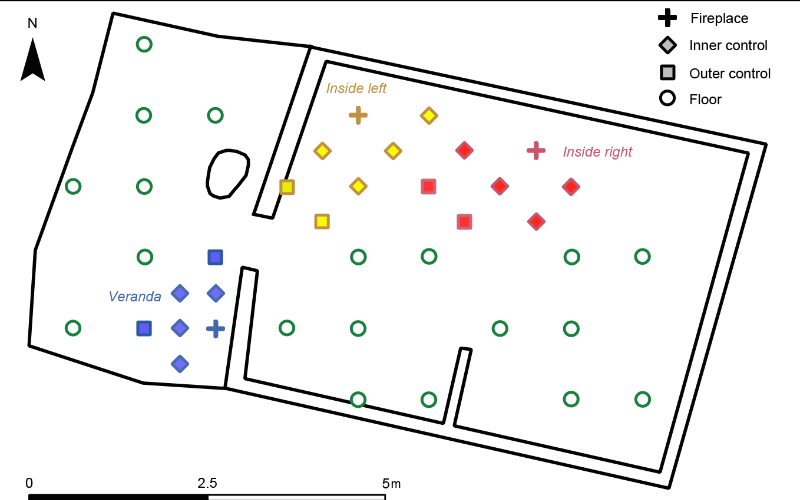
\includegraphics[width=15cm]{figures/figure_samples}
    \caption{Map of the domestic space analysed with indication of samples location and the three different fireplaces with their respective control samples color-coded}.
    \label{fig:samples}
  \end{center}
\end{figure*}

\section{Results}
\label{sec:3}
A summary of the phytoliths and geochemistry results are given in table 1. As mentioned in section 3 (Material and Methods, Samples) extensive material is available for downloading from an online open access repository.
\subsection{Phytoliths}
\label{subsec:3.1}
\paragraph{Concentration}
Overall concentration differences amongst the samples are present as indicated by the MANOVA results (p\textless{0.05}, see supplementary material) however, when looking at each single fireplace no significant differences are highlighted between the fireplace and its control samples by ANOVA (p=0.2 for Inside\_right; 0.7 for Inside\_left and 0.5 for Veranda). Nevertheless, clear patterns emerge from the analysis of concentration: general floor samples have higher concentration and variability than fireplaces (including their control samples, see figure \ref{fig:box}). Among the fireplaces the one currently in use inside the house (Inside\_right) is the one that present the lowest concentration of phytoliths (figure \ref{fig:conc}). 

\begin{figure*}[ht!]
  \begin{center}
    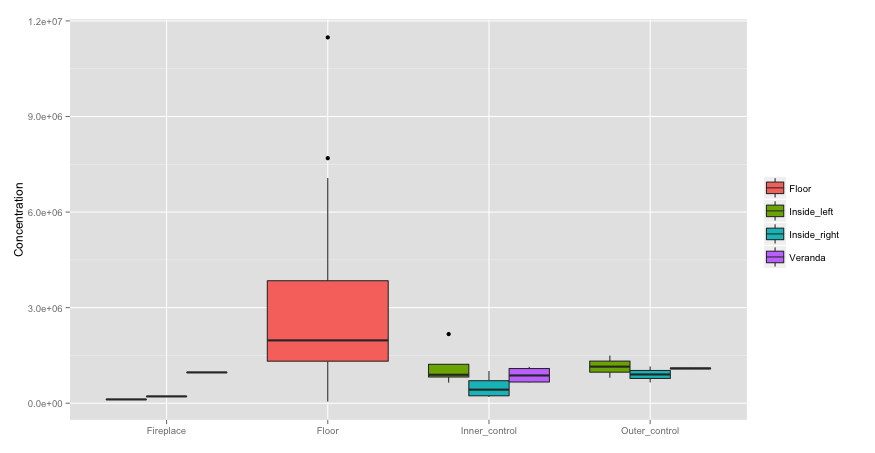
\includegraphics[width=15cm]{figures/concentration_fp}
    \caption{Differences in phytolith concentrations between the groups of samples under study. Notice that the three fireplaces (Inside\_left, Inside\_right and Veranda) include both the fireplace and the control samples}.
    \label{fig:box}
  \end{center}
\end{figure*}

\begin{figure*}[ht!]
  \begin{center}
    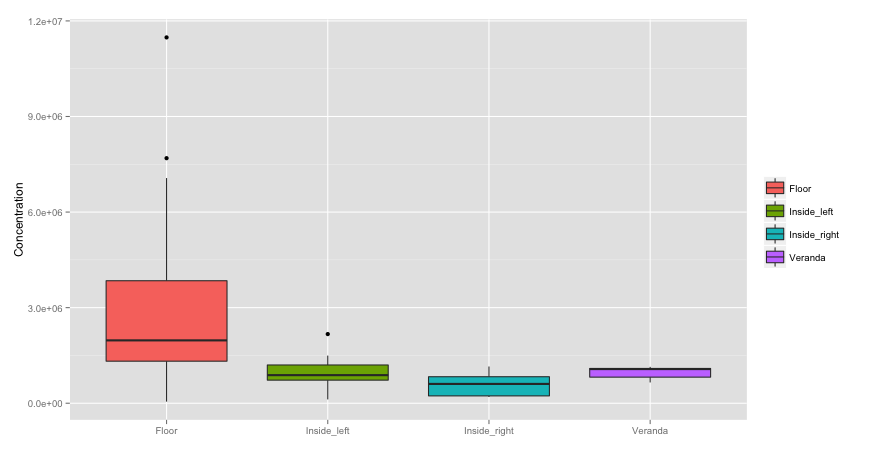
\includegraphics[width=15cm]{figures/concentration_groups}
    \caption{Differences in phytolith concentrations within the groups of samples under study. Notice that the three fireplaces (Inside\_left, Inside\_right and Veranda) display a concentration much lower than those of floor samples and of the outer controls and that Floors have a much higher variability than the control samples}.
    \label{fig:conc}
  \end{center}
\end{figure*}

\begin{table}[]
\centering
\caption{Summary of the phytoliths and geochemical analysis. All values, except phytolith concentration are given as percentages.}
\label{table:1}
\rotatebox{90}{
	\begin{tabular}{llcccccccc}
 &  & \multicolumn{6}{c}{Phytoliths} & \multicolumn{2}{c}{Elements} \\
Area & Type & \multicolumn{1}{l}{Concentration} & \multicolumn{1}{l}{Graminoids\_leaf/culm} & \multicolumn{1}{l}{Graminoids\_inflorescence} & \multicolumn{1}{l}{Herbaceous\_indet} & \multicolumn{1}{l}{Woody\_species} & \multicolumn{1}{l}{Indet} & \multicolumn{1}{l}{Dung} & \multicolumn{1}{l}{Wood} \\
Veranda & Outer\_control & 1092066 & 6.63 & 1.78 & 86.25 & 2.27 & 3.07 & 55.52 & 44.48 \\
 & Inner\_control & 883792 & 8.07 & 3.35 & 80.12 & 2.06 & 6.40 & 55.41 & 44.59 \\
 & Fireplace & 966850 & 10.90 & 4.67 & 77.88 & 1.25 & 5.30 & 54.09 & 45.91 \\
Inside\_left & Outer\_control & 1148302 & 7.18 & 3.19 & 81.50 & 1.75 & 6.38 & 57.09 & 42.91 \\
 & Inner\_control & 1151112 & 13.04 & 2.81 & 76.42 & 1.33 & 6.40 & 57.30 & 42.70 \\
 & Fireplace & 119056 & 19.15 & 3.65 & 70.82 & 0.00 & 6.38 & 60.29 & 39.71 \\
Inside\_right & Outer\_control & 902626 & 7.50 & 2.00 & 86.67 & 0.50 & 3.33 & 56.92 & 43.08 \\
 & Inner\_control & 514262 & 9.98 & 1.98 & 80.05 & 1.32 & 6.68 & 58.29 & 41.71 \\
 & Fireplace & 213991 & 9.62 & 2.88 & 76.60 & 0.32 & 10.58 & 61.08 & 38.92 \\
Floor &  & 2981254 & 12.87 & 3.14 & 76.73 & 1.86 & 5.39 & 57.45 & 42.55
\end{tabular}
}
\end{table}

\paragraph{Taphonomy}
Considering the short deposition time, taphonomy should not have had a primary impact on the assemblages under study. However, repetitive sweepings of the floor can damages to the phytoliths and changes in the assemblages. An analysis of the average number of cells per silica skeleton indicates that physical breakage is slightly higher in the two fireplaces in use (2.37 in the veranda and 2.08 in the inner hearths) than in the general floor sediments (3.27) and in the fireplace not currently in use (5.98).

\paragraph{Morphological analysis}
A total of 37 different morphotypes were identified during the analysis and subsequently grouped for the specific aims of this work into the taxonomical groups specified above. All samples presented over 70\% of indeterminate herbaceous morphotypes, which clearly indicate that grasses represent the primary input of phytoliths in the samples. The three fireplaces present a similar morphological composition, except in respect to woody dicotyledonous morphotypes which are higher in the veranda fireplace and not present in the two interior hearths (figure \ref{fig:morpho}). The three fireplaces show different trends in morphological composition in respect to their controls: a) the Inside\_right fireplace, shows lower percentages of grass leaf/cul, grass inflorescence and woody species morphotypes than its controls; b) the Inside\_left hearth, a higher quantity of leaf/culm, lower values of woody dicotiledonous and inflorecscence higher than the inner controls but lower than the outer controls; and c) the Veranda fireplace higher concentration of leaf/culm and inflorescence morphotypes, but lower values of woody dicotyledonous in respect to both inner and outer controls. The two fireplaces in use (Veranda and Inside\_right) show a difference in the distribution of woody dicotyledonous morphotypes within the control samples, which are more concentrated in the inner control than in the outer control samples in the case of the hearth inside the house and vice versa in the veranda fireplace. Inflorescence morphotypes are higher in floor samples, and present values similar to the control samples (inner and outer) of the inner fireplace not in use.

\begin{figure*}[ht!]
  \begin{center}
    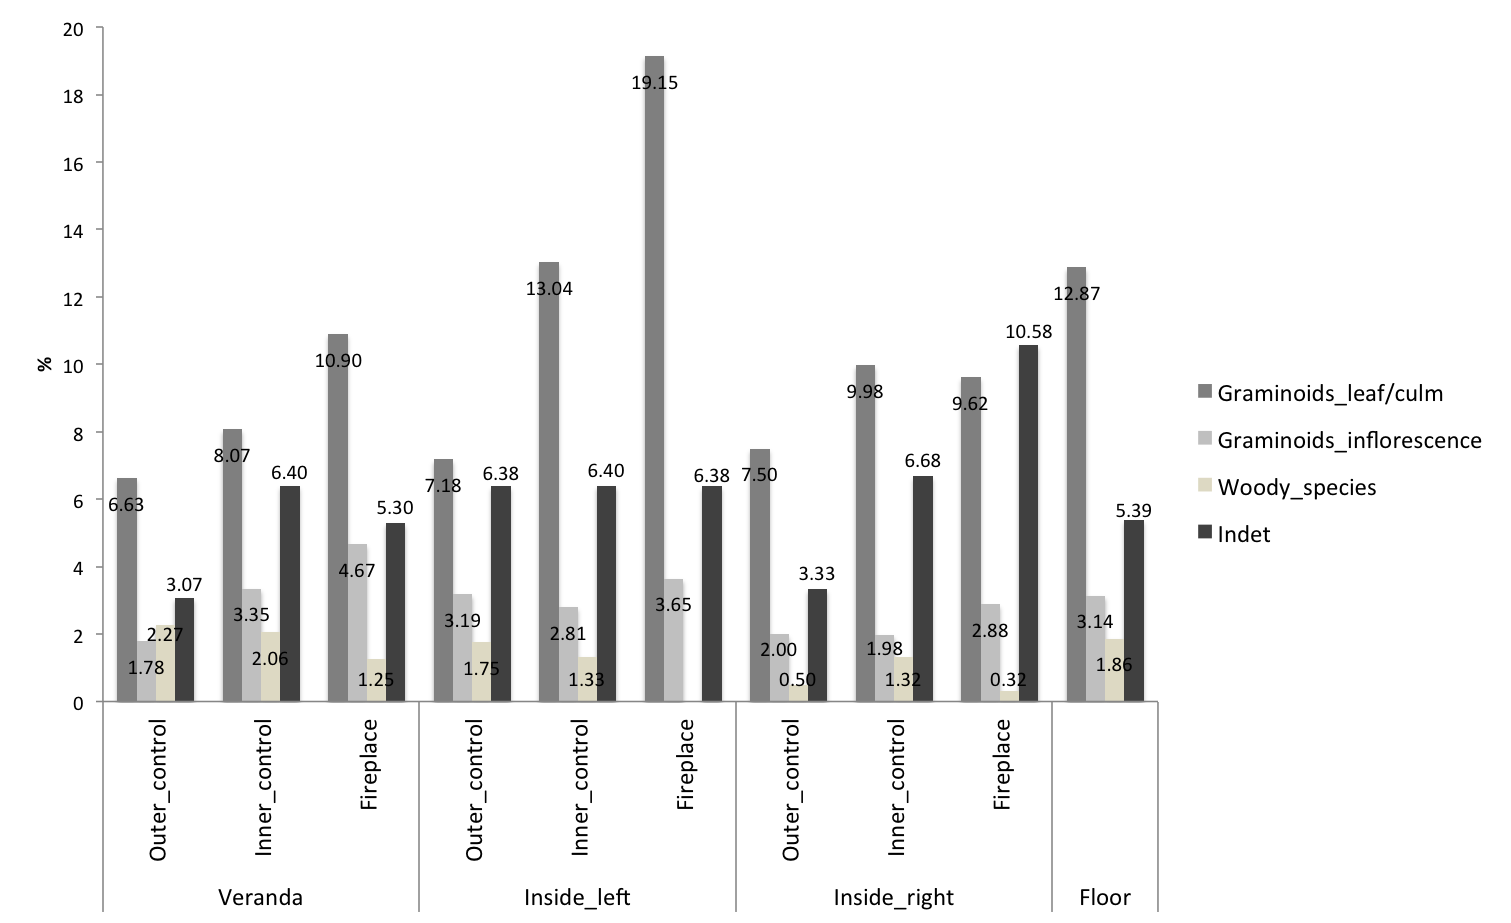
\includegraphics[width=15cm]{figures/fp_bar}
    \caption{Bar chart of the morphotypological groups observed in the samples. Indeterminate herbaceous type have been excluded as they constituted over 70\% of the samples impairing the understanding of differences.}
    \label{fig:morpho}
  \end{center}
\end{figure*}

\subsection{Multi-element geochemistry}
\label{subsec:3.2}
Figure \ref{fig:chem} shows the composition of samples in relation to the dung and wood groups. In accordance to previous results, the fireplace situated in the veranda shows a peak of dung signature with respect to the other two fireplaces. Interestingly this fireplace also shows the highest peak in wood ash elements. To be noticed the difference between the fireplaces and their control samples: in the case of the two inner fireplaces, elements are less concentrated in the fireplace than in the control samples whereas the veranda hearth has higher values than its control samples. In general, control samples present the same levels in both dung and wood ash elements than the floor samples (both inside the house and in the veranda).

\begin{figure*}[ht!]
  \begin{center}
    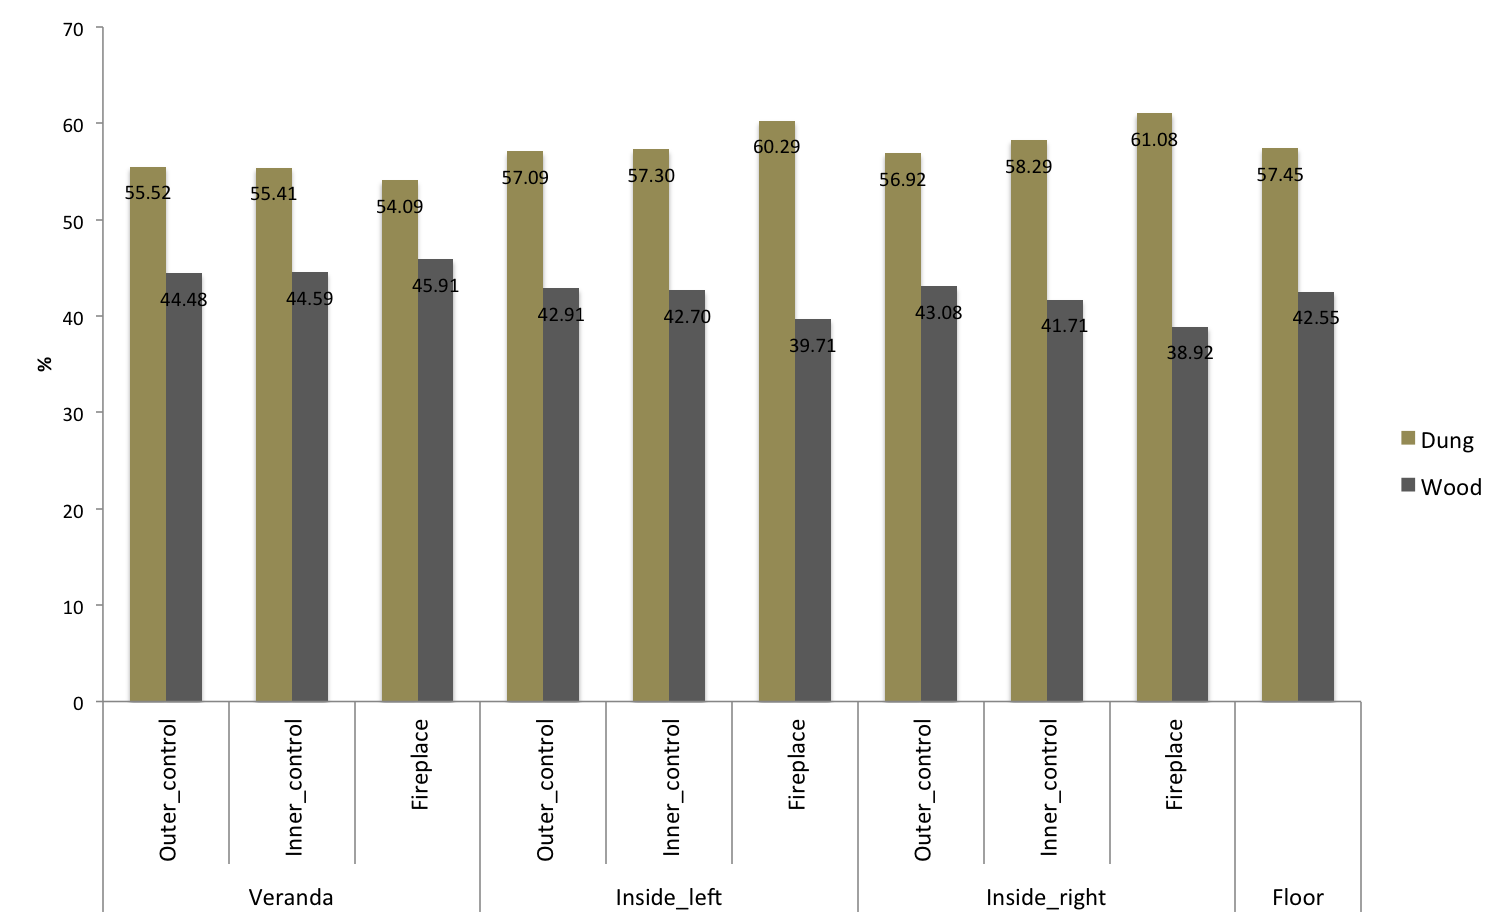
\includegraphics[width=15cm]{figures/chem_bar}
    \caption{Bar chart of the wood and dung chemical groups}
    \label{fig:chem}
  \end{center}
\end{figure*}

\subsection{Integration of data}
\label{subsec:3.3}	
Principal Component Analysis was performed only on phytoliths and on phytolith and chemical elements groups, both including the dung reference collection. However, analyses performed including fresh and ashed dung samples from reference collection showed that the latter are clearly different from the ethnographic samples both in phytolith composition (figure \ref{fig:dungPCA}a) and in phytolith and chemical composition (figure \ref{fig:dungPCA}b). Further analyses were then performed excluding the reference collection of dung. These showed that there is some overlap between the four groups of samples (fireplaces, inner control, outer control and general floor). However, phytoliths alone (figure \ref{fig:PCA}a) discriminate fireplaces (especially the two inner ones) from other samples, whereas phytoliths and chemical elements results (figure \ref{fig:PCA}b) contribute to a full discrimination between the fireplaces, also in the case of the Veranda fireplace. Another important results is the clear separation between the fireplace samples and the outer controls, whereas the inner control cluster extremely close to the fireplaces.

\begin{figure*}[ht!]
  \begin{center}
    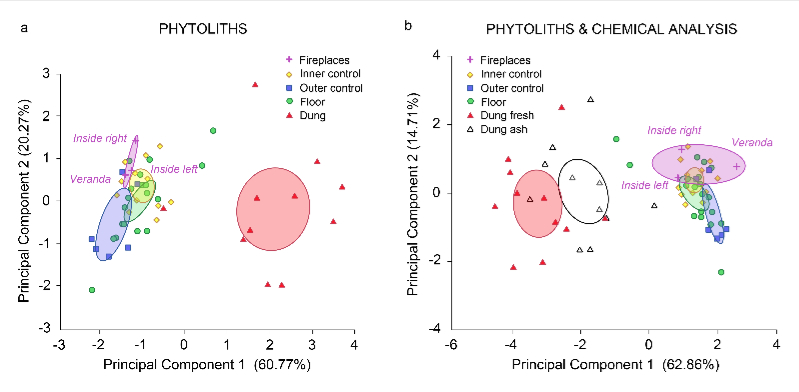
\includegraphics[width=15cm]{figures/PCA_dung}
    \caption{Plot of the PCA performed on phytolith (a) and phytoliths and chemical data (b) including both ethnographic and dung reference collection samples (ellipses are drawn automatically around the barycentre of the groups).}
    \label{fig:dungPCA}
  \end{center}
\end{figure*}


\begin{figure*}[ht!]
  \begin{center}
    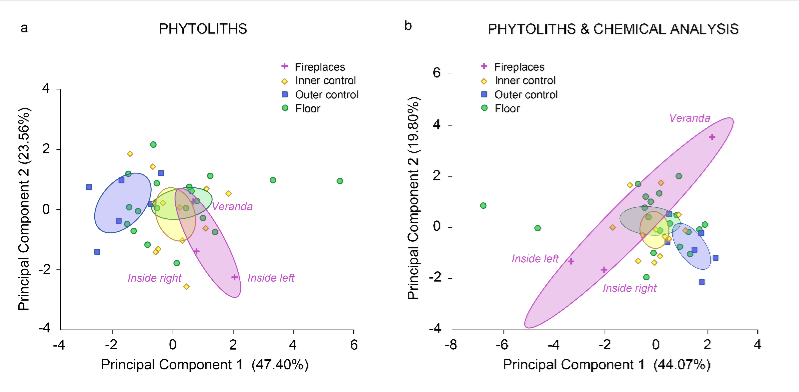
\includegraphics[width=15cm]{figures/PCA}
    \caption{Plot of PCA performed on phytolith (a) and phytolith and chemical data (b) from the ethnographic samples only, excluding the dung reference collection samples (ellipses are drawn automatically around the barycentre of the groups)}.
    \label{fig:PCA}
  \end{center}
\end{figure*}



\section{Discussion}
\label{sec:4}
Fire is one of the fundaments of human life and fuel one of the biggest issues of the modern wold. Alternative fuels were important not only in the past, but continue to be a fundamental resources for rural households \citep{Viswanathan2005}: in India, one of the most recent estimates on the value of dung as fuels rounded at 1.5 billions dollars \citep{Harris2000}. With the current trend in climate chage at the global level and the increase in pressure on vegetation, it is to be expected that the value of alternative fuels will only increase. For this reason, unravelling the strategies behind fuel exploitation and use that past society have put in place to deal with scarcity can offer precious hints on how to deal with some of the challenges of our way of life. In this perspective, it is pivotal for archaeologist to rely on robust and secure analytical and interpretative models when addressing the study of fuel use in the past. Wood charcoal remains have been one of the primary sources of information on past fuel use. However, in many archaeological contexts charcoal remains are not present, either due to post-depositional taphonomic processes or because wood was not the primary source of fuel. This is often the case in arid and semi-arid areas, where trees are scarce and alternative fuel sources need to be exploited, such as dung (often in the form of dung cakes) and crop-processing byproducts.\par
In this work we show the value of ethnography as a support for data interpretation and methodological improvement. Previous work conducted in the same context had highlighted possible interpretation problems on an otherwise innovative and powerful methodology \citep{Rondelli2014}. With the present work we showed that a multi-proxy approach with the integration of phytoliths analysis and the application of multivariate statistics, those challenges can be solved. The high concentration of Graminoids phytoliths in all samples, together with the predominance of graminoids leaf/culm morphotypes, with small inputs from Graminoids inflorescences as well as woody taxa highlight, on one side, the homogeneity of the base material (dung, see \citealt{Lancelotti2012}), which is used in the study-context as main component of structures (\emph{i.e.}, floors and walls). Therefore it is to be expected, as mirrored in the results, that both phytoliths and chemical elements display a high level of dung signatures (table \ref{table:1} and figures \ref{fig:morpho} and \ref{fig:chem}). Previous studies conducted on the dung reference material had showed that phytolith and chemical composition of the dung cakes was independent on their site of collection \citep{Lancelotti2012}. Therefore, the comparison of results with modern dung reference collection was performed assuming that the floor samples will be closer to the fresh dung and the fireplace samples where dung was used as fuel will be cluster together with the ashed dung. However, reference samples did not cluster with any of the ethnographic samples, suggesting that that the stronger signal, both in chemical elements and phytolith is provided by a source different than dung. Nevertheless, there are important anomalies (i.e., discontinuities in the data) that provide anchors for interpretation of the firing activities. It is important to notice that, in the case of phytoliths from within the fireplace (centre of the structure), the actual use of the hearth plays a much important role in the formation of the phytolith assemblage than the fuel used. In other words, the phytolith assemblage recovered from inside the fireplaces represent a short snapshot of the firing practices and indicate just the last, or few lasts, burning episodes (a fact that is valid for, and has been previously observed in wood charcoal studies; see for example \citealt{Chabal1997}). In this respect, the hearth located in the veranda, which was actually the one in use in the days when sampling was carried out, presented the highest value of woody morphotypes even though the normal fuel used here is a mixture of prevalently dung. Both the short-term nature of the fireplace deposit and the mixture of dung and wood fuel used in the veranda, are corroborated by the chemical analyses and the high peak of both dung and wood ash elements found in this sample. As both groups include P, these high peaks are determined by the very high concentration of this element in the sample collected in the external fireplace.\par
In order to clearly understand fuel practices we suggest that, as phytoliths are concerned, an important role is played by the samples immediately surrounding the fireplace. For example, interviews conducted with the family occupying the house indicated a preferential use of wood in the two hearths located inside the house (Inside\_right and Inside\_left). The fireplace sample showed no or next to no woody dicotyledon morphotypes, whereas the control samples (both inner and outer) present a relatively high percentage. This particular deposition patterns are to be related to the high probability of ash dispersing in the surrounding of the fireplace either during cooking or during the periodical cleaning of the hearths. Being these repetitive activities that continuously deposit microremains on the floor, an accumulation is produced that leave a clear signature in the record. Indeed, even if the floor is also cleaned periodically, this activity affects the entire surface of the floor. Therefore, the anomalies in the deposition of phytoliths are, not only preserved, but also increased by the sweeping activities that contribute to spread the fuel residues around the fireplace itself.\par
Multivariate statistics performed on phytoliths and on both phytolith and chemical data suggest that, although a certain degree of separation exists when all the samples' groups are considered together, no statistical differences are to be found between each fireplace and its controls. This corroborates the suggestion expressed above that the samples surrounding the actual firing contexts can help in the identification of fuel practices. PCAs indicate, however, that just the controls closer to the fireplace are representative of the fuel used as the outer controls tend to form separate cluster that do not overlap with the fireplaces.\par
\TODO{Add something on archaeology}.


\section{Conclusions}
\label{sec:5}
We maintain that a quantitative and multi-proxy approach is necessary to correctly identify traces of fuel alternative to wood in archaeological contexts. Moreover, we propose that ethnography can be a powerful source of information, not in the sense of tracing a direct parallel between modern and past practices, but as a context in which to test hypotheses and methodologies. Indeed, only by comparing the results of our analytical work against contexts that are secure and on which we have exact information, can we fine-tune our interpretation of analytical results. This study showed how the integration of phytoliths and geochemical elements, can contribute to our definition of fuel practices and how, in order to really grasp the full extent of fuel use in domestic contexts, researchers need to take into consideration not only the fireplace context but also the samples immediately surrounding it.

\section{Acknowledgements}
\label{sec:acknowledgements}
All authors belong to the Complexity and Socio-Ecological Dynamics (CaSEs) Research Group, a Grup de Recerca Emergent (SGRe-1417) of the Generalitat de Catalunya, coordinated by Marco Madella. This research was carried out within the framework of the North Gujarat Archaeological Project, which received fundings from the Ministry of Economy and Competitiveness (HAR2010-16052) and the Ministry of Education, Culture and Sport through the program \textit{Ayudas para Proyectos Arqueológicos en el Exterior 2009-2010}. JJGG was supported by a JAE PreDOC PhD scholarship (Spanish National Research Council and European social Fund). The authors are extremely grateful to all their Indian colleagues, especially Ajithprasad P. and Charusmita Gadekar for their invaluable help in the field. We also want to thank warmly Sakti-ji, Nema-ji, Puri Sonal and Nita for welcoming us in their home, letting us make holes in their floor and being very patient with all our questions.

\section{References}

%% References with bibTeX database:

\bibliographystyle{model2-names}
\bibliography{impr_biblio}

\end{document}